%----------------------------------------------------------------------------
\chapter{Kísérlet}\label{sect:kiserlet}
%----------------------------------------------------------------------------

\texttt{+++ bevezeto a fejezethez +++}

%Szöveg.

%,,,,,,,,,,,,,,,,,,,,,,,,,,,,,,,,,,,,,,,,,,,,,,,,,,,,,,,,,,,,,,,,,,,,,,,,,,,,
\section{Módszerek összehasonlítása}\label{sect:modsz_osszehasonlitas}
%,,,,,,,,,,,,,,,,,,,,,,,,,,,,,,,,,,,,,,,,,,,,,,,,,,,,,,,,,,,,,,,,,,,,,,,,,,,,

\texttt{+++ miert BLOB-os keresest valasztottam Hough vagy Optical flow helyett? +++}

%,,,,,,,,,,,,,,,,,,,,,,,,,,,,,,,,,,,,,,,,,,,,,,,,,,,,,,,,,,,,,,,,,,,,,,,,,,,,
\section{Feldolgozási folyamat}\label{sect:feld_folyamat}
%,,,,,,,,,,,,,,,,,,,,,,,,,,,,,,,,,,,,,,,,,,,,,,,,,,,,,,,,,,,,,,,,,,,,,,,,,,,,

\texttt{+++ milyen kepfeldolgozasi (elo)feldolgozas kell a detektalashoz? +++}

%............................................................................
\subsection{Pupillakövetés}\label{sect:pupillakov}
%............................................................................

\texttt{+++ feldolgozasi lepesek a koveteshez +++}

%............................................................................
\subsection{Kalibráció, leképezés}\label{sect:kalibracio}
%............................................................................

\texttt{+++ kalibrálás + kepernyo-koordinataba kepzes +++}

%,,,,,,,,,,,,,,,,,,,,,,,,,,,,,,,,,,,,,,,,,,,,,,,,,,,,,,,,,,,,,,,,,,,,,,,,,,,,
\section{Kísérletek}\label{sect:kiserletek}
%,,,,,,,,,,,,,,,,,,,,,,,,,,,,,,,,,,,,,,,,,,,,,,,,,,,,,,,,,,,,,,,,,,,,,,,,,,,,

\texttt{+++ leiras hogy miert ezekkel probaltam ki +++}

%............................................................................
\subsection{Pszichológiai bemutató}\label{sect:pszicho}
%............................................................................

A rendszer működését úgy demonstráltam, hogy végrehajtottam Alfred L. Yarbus orosz pszichológus 1967-es tanulmánya egy részletét. A kísérletben a kutatók azt bizonyították be, hogy a tesztalanyoknak előzetesen különböző kérdéseket feltéve, a kérdések jelentősen befolyásolták egy kép részleteinek vizsgálatát ahhoz képest, ha csak ,,szabadon'' nézegették azt. A teszteredményeket összefoglaló kép -- mint az egyik első a témával foglalkozó eredmény -- jól ismert a tekintetkövetéssel foglalkozók körében, ez látható a \figref{yarbus} ábrán.

\begin{figure}[!ht]
\centering
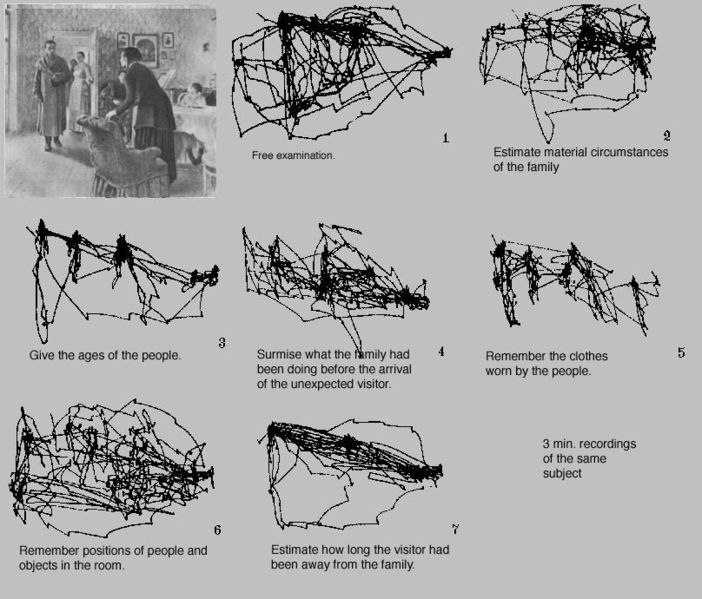
\includegraphics[width=140mm, keepaspectratio]{figures/yarbus.jpg}
\caption{Yarbus '67-es kísérletének eredménye}
\label{fig:yarbus}
\end{figure}

Látható, hogy a kísérlet végrehajtásához szükség volt a tekintet követésére. Ekkor még a kornak megfelelően nem álltak rendelkezésre kifinomult módszerek: az alanyokat egy meglehetősen kényelmetlen acélszerkezethez rögzítve vizsgálták. A bemutató alkalmazásomban arra kerestem a választ, hogy lehetséges-e hasonló méréseket elvégezni az általam fejlesztett rendszerrel.

\bigskip

Az általam tesztelt alanyoknak a következő kérdésekre kellett válaszolniuk a tesztkép (Repin: Váratlan utazó) rövid vizsgálata után. A vizsgálatot minden kérdésben 200 beérkezett érvényes mérési pontig folytattam, ez a felhasznált webkamera, illetve a feldolgozási sebesség mellett nagyjából kérdésenként 15--20 másodpercet vett igénybe.

\begin{enumerate}
 \item szabad nézelődés
 \item ,,Milyen anyagi körülmények között él a család?''
 \item ,,Adja meg az egyes szereplők életkorát!''
 \item ,,Mit csinálhattak a szereplők, mielőtt az utazó betoppant?''
 \item ,,Milyen ruhát viselnek a kép szereplői?''
 \item ,,Próbáljon megjegyezni minél több strukturális részletet (személyek, tárgyak pozíciója)!''
 \item ,,Mennyi ideig lehetett távol az utazó a családtól?''
\end{enumerate}

A kérdésekre nem volt jó, vagy rossz válasz, a kísérlet minden alanynál csak a feladatnak megfelelő figyelmi területek változását vizsgálja. A vizsgálatom eredménye a \figref{eredmeny} ábrán követhető.

\begin{figure}[!ht]
\centering
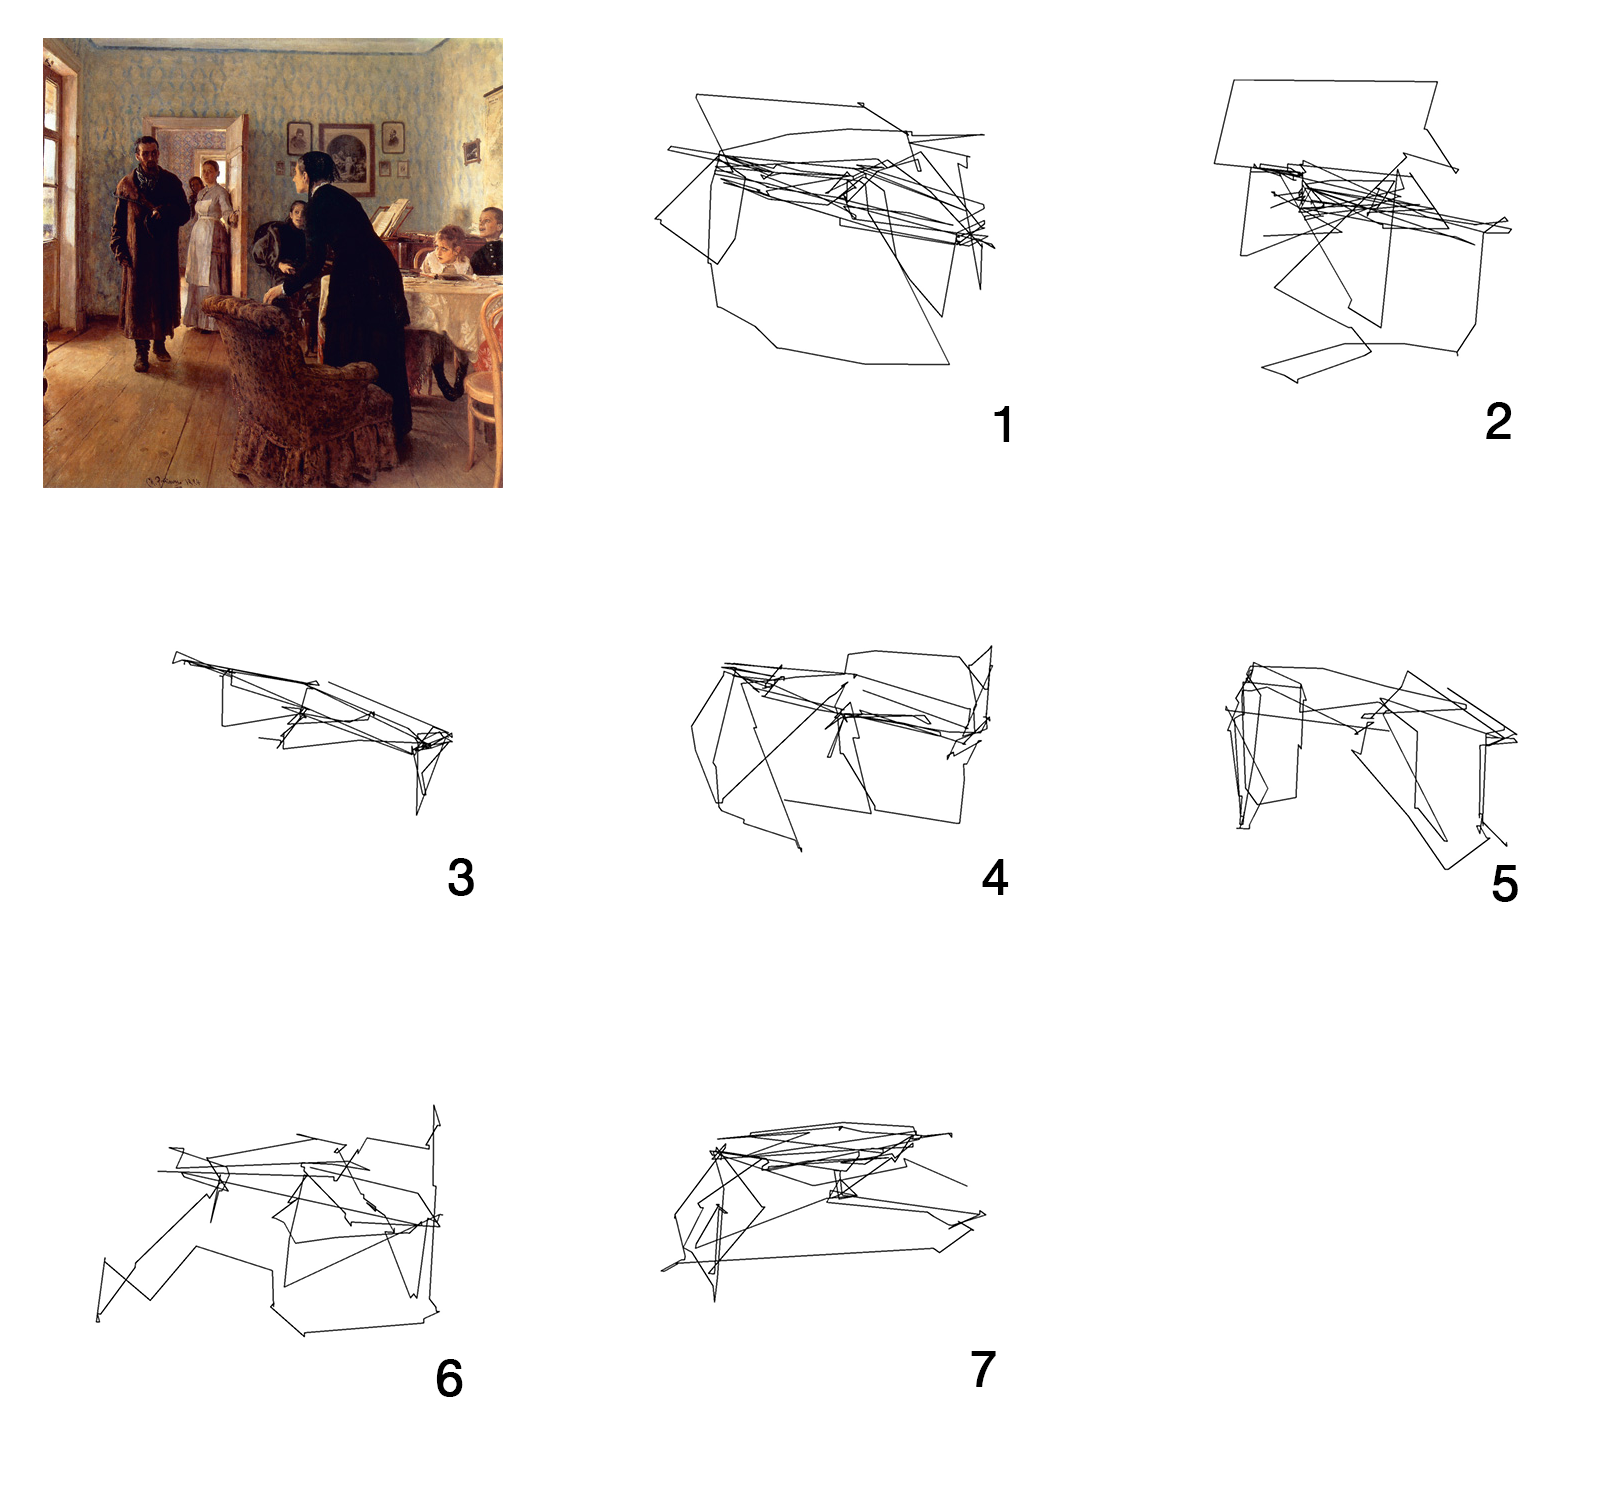
\includegraphics[width=140mm, keepaspectratio]{figures/yarbus_eredmeny.png}
\caption{Eredmények a saját rendszerrel}
\label{fig:eredmeny}
\end{figure}

Látható -- bár ez nem volt feltétel -- hogy a mérési eredmények ezen alany esetén meglehetősen jól fedik Yarbus tesztalanyának eredményeit. Az viszont mindenképpen kijelenthető, hogy szignifikáns különbség van az ábra első (szabad nézelődés), valamint többi része között. Nem célom a kísérlet pszichológiai eredményeit értékelni, az viszont bizonyos, hogy a rendszer hasonló kísérletek elvégzését támogatja.

%,,,,,,,,,,,,,,,,,,,,,,,,,,,,,,,,,,,,,,,,,,,,,,,,,,,,,,,,,,,,,,,,,,,,,,,,,,,,
\subsection{Webergonómiai bemutató}\label{sect:web}
%,,,,,,,,,,,,,,,,,,,,,,,,,,,,,,,,,,,,,,,,,,,,,,,,,,,,,,,,,,,,,,,,,,,,,,,,,,,,

Ahogyan dolgozatom első fejezetében már említettem, a tekintet követése a webergonómia területén is fontos kísérletek elvégzésére ad lehetőséget. A rendszer ilyen irányú képességeit demonstrálandó, elkészítettem az pszichológiai kísérlet adatait hőtérképen (heat map) megjelenítő funkciót is, ennek eredménye egy tesztképre a \figref{heatmap} ábrán látható.

\begin{figure}[!ht]
\centering
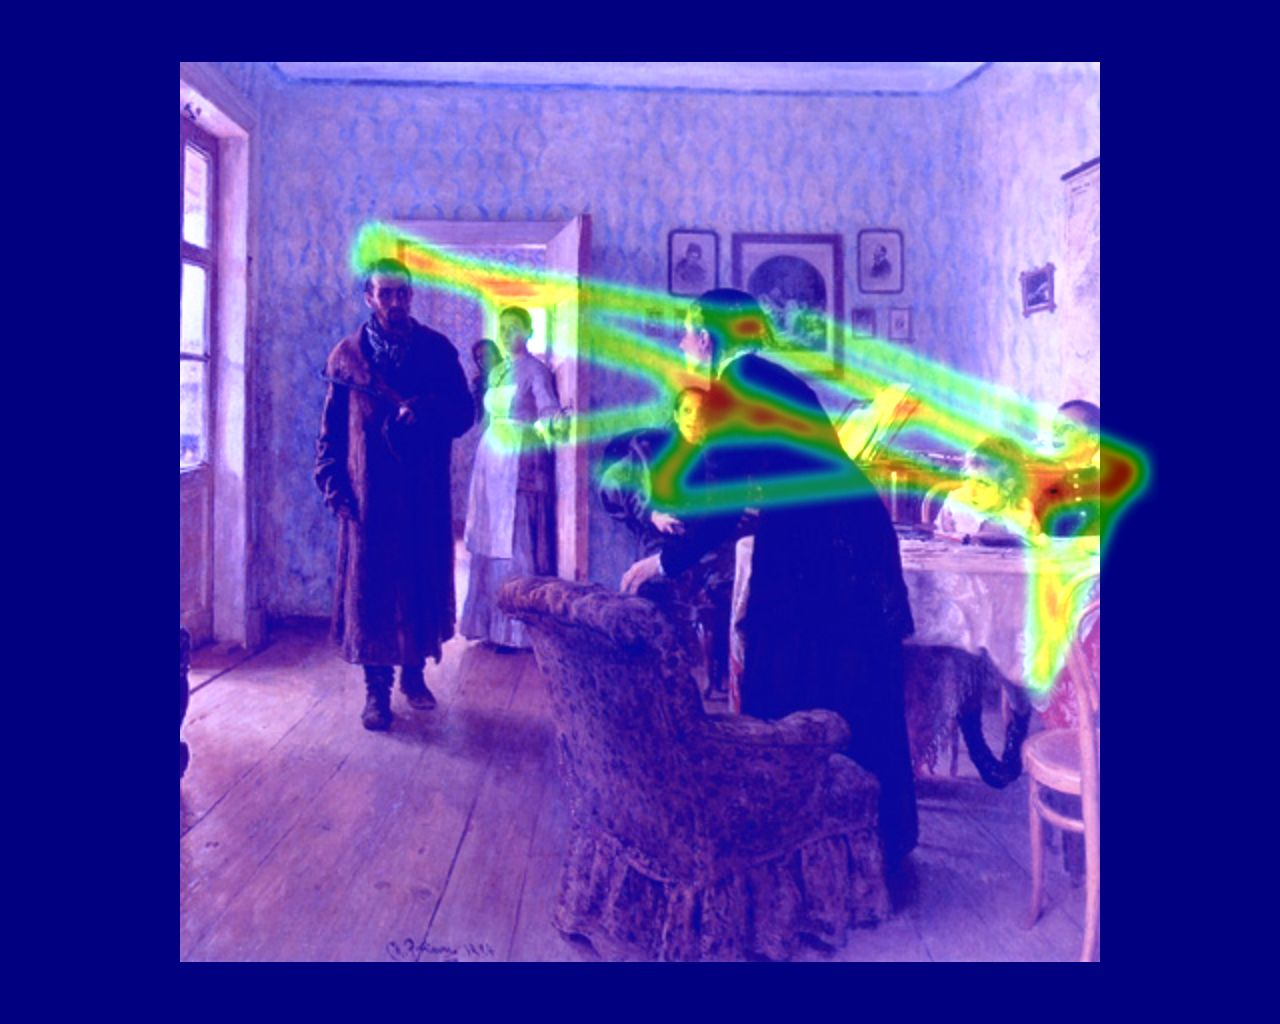
\includegraphics[width=100mm, keepaspectratio]{figures/heatmap.jpg}
\caption{Hőtérképes megjelenítés a pszichológiai teszt egy adathalmazára (,,Adja meg a szereplők életkorát!'')}
\label{fig:heatmap}
\end{figure}

Minden vizsgálatban célszerű a lehető leginkább informatív megjelenítést választani a rendelkezésre álló adathalmaz alapján. A képen egyre pirosabb színnel jelöltem a kép frekventáltan vizsgált területeit, például egy webergonómiai vizsgálatban az adatok effajta vizualizációja lehet a legcélszerűbb.

\bigskip

\texttt{+++ meg 1-2 bekezdes +++}

%,,,,,,,,,,,,,,,,,,,,,,,,,,,,,,,,,,,,,,,,,,,,,,,,,,,,,,,,,,,,,,,,,,,,,,,,,,,,
\section{Összefoglalás}\label{sect:kiserlet_osszefoglalas}
%,,,,,,,,,,,,,,,,,,,,,,,,,,,,,,,,,,,,,,,,,,,,,,,,,,,,,,,,,,,,,,,,,,,,,,,,,,,,

\texttt{+++ osszefoglalas a kiserletekrol +++}